\documentclass[t]{beamer}
\usepackage{mathtools}
\usepackage{tikz}
\usepackage{pgfplots}
\usepackage{ifthen}
\usepackage{calc}
\usepackage{datatool}
\usepackage{datapie}
\usetikzlibrary{arrows,backgrounds,shapes,matrix,positioning,fit}
\usetikzlibrary{calendar}
\newcommand{\argmax}{\operatornamewithlimits{argmax}}
\newcommand{\argmin}{\operatornamewithlimits{argmin}}
\newcommand{\wt}{\operatornamewithlimits{wt}}

\mode<presentation>
{
  \usetheme{Singapore}
  %\useoutertheme{infolines} % Showing only current section in navigation
  \setbeamertemplate{headline}{}  % Empty headline
  \setbeamertemplate{footline}[frame number]  % Getting rid of footer items except slide number
  \setbeamercovered{invisible}
  \beamertemplatenavigationsymbolsempty % Getting rid of navigation bullets at the bottom
}
\usepackage[english]{babel}
\usepackage[latin1]{inputenc}
\usepackage{times}
\usepackage[T1]{fontenc}

\title[EE 703 DMT]{EE 703 Digital Message Transmission}
\author[Saravanan V]
{
  Saravanan Vijayakumaran\\
  \href{mailto:sarva@ee.iitb.ac.in}{sarva@ee.iitb.ac.in}
}
\institute[IIT Bombay]
{
  Department of Electrical Engineering\\
  Indian Institute of Technology Bombay
}
\date{July 18, 2013}

\begin{document}

\begin{frame}
  \titlepage
\end{frame}

\begin{frame}{Course Details}
  \begin{description}
    \item[Instructor] Saravanan Vijayakumaran
    \item[Office] EE 122B (Opposite PC Lab)
    \item[Schedule] Slot 1
    \item[Location] EEG 002
    \item[Webpage] \url{http://www.ee.iitb.ac.in/~sarva/EE703/Autumn2013.html}
    \item[Forums] \url{https://piazza.com/iit_bombay/other/ee703}
  \end{description}
\end{frame}

%% Database for marks distribution
\DTLnewdb{gradingpolicy}
\DTLnewrow{gradingpolicy}
\DTLnewdbentry{gradingpolicy}{Name}{Endsem}
\DTLnewdbentry{gradingpolicy}{Points}{45}
\DTLnewrow{gradingpolicy}
\DTLnewdbentry{gradingpolicy}{Name}{Midsem}
\DTLnewdbentry{gradingpolicy}{Points}{30}
\DTLnewrow{gradingpolicy}
\DTLnewdbentry{gradingpolicy}{Name}{Quizzes}
\DTLnewdbentry{gradingpolicy}{Points}{15}
\DTLnewrow{gradingpolicy}
\DTLnewdbentry{gradingpolicy}{Name}{Assignments}
\DTLnewdbentry{gradingpolicy}{Points}{10}
%% End database

\begin{frame}{Grading Policy}
  \begin{figure}
  \centering
  \setcounter{DTLpieroundvar}{0}
  \DTLpiechart{variable=\points,outerlabel=\name,innerratio=0.7,outerratio=1.1,innerlabel={\DTLpiepercent\%}}
              {gradingpolicy}
              {\points=Points,\name=Name}
  \end{figure}

  \begin{itemize}
    \item Quizzes (Best two out of three)
    \item Relative grading
    \item For AU, score $\geq$ CC
  \end{itemize}
\end{frame}

\begin{frame}{Reference Books}
  \begin{itemize}
    
    \item \textit{Fundamentals of Digital Communication}, Upamanyu Madhow, 2008
    \item \textit{Digital Communications}, John G. Proakis and Masoud Salehi, 2008 (5th Edition)
  \end{itemize}
\end{frame}


\begin{frame}{Digital Communication Systems}
  \begin{figure}
  \centering
  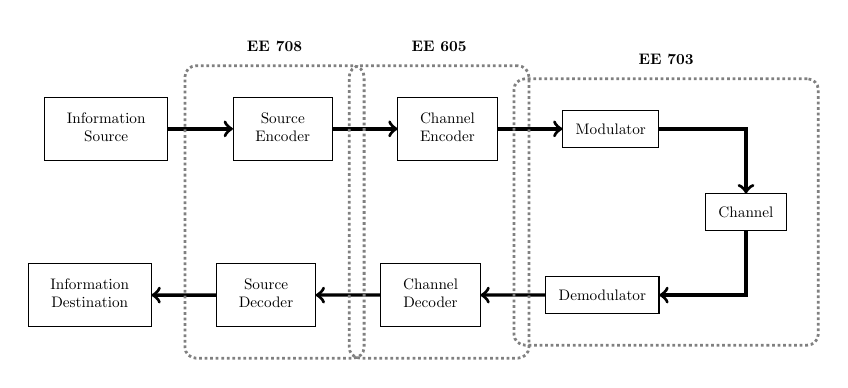
\begin{tikzpicture}[scale=0.55,transform shape]
  \tikzstyle{rectblock}=[rectangle, draw, inner sep=3mm]
  \node[rectblock] (Source) {\begin{tabular}{c} Information\\
                                                Source
                             \end{tabular}};
  \node[rectblock, right=1.5cm of Source] (Source Encoder) {\begin{tabular}{c}Source\\
                                                                             Encoder
                                                           \end{tabular}};
  \node[rectblock, right=1.5cm of Source Encoder] (Channel Encoder) {\begin{tabular}{c}Channel\\
                                                                             Encoder
                                                           \end{tabular}};
  \node[rectblock, right=1.5cm of Channel Encoder] (Modulator) {Modulator};
  \node[rectblock, below right=1.5cm of Modulator] (Channel) {Channel};
  \node[rectblock, below left=1.5cm of Channel] (Demodulator) {Demodulator};
  \node[rectblock, left=1.5cm of Demodulator] (Channel Decoder) {\begin{tabular}{c}Channel\\
                                                                               Decoder
                                                             \end{tabular}};
  \node[rectblock, left=1.5cm of Channel Decoder] (Source Decoder) {\begin{tabular}{c}Source\\
                                                                               Decoder
                                                             \end{tabular}};
  \node[rectblock, left=1.5cm of Source Decoder] (Destination) {\begin{tabular}{c} Information\\
                                                                                   Destination
                                                                \end{tabular}};
  \draw [->,very thick] (Source) -- (Source Encoder);
  \draw [->,very thick] (Source Encoder) -- (Channel Encoder);
  \draw [->,very thick] (Channel Encoder) -- (Modulator);
  \draw [->,very thick] (Modulator) -| (Channel);
  \draw [->,very thick] (Channel) |- (Demodulator);
  \draw [->,very thick] (Demodulator) -- (Channel Decoder);
  \draw [->,very thick] (Channel Decoder) -- (Source Decoder);
  \draw [->,very thick] (Source Decoder) -- (Destination);
  \tikzset{dotted/.style={draw=black!50!white, line width=1pt,
                         dash pattern=on 1pt off 1pt,
                         inner sep=4mm, rectangle, rounded corners}};
  \pause
  \node (EE708 dotted box) [dotted, fit = (Source Encoder) (Source Decoder)] {};
  \node at (EE708 dotted box.north) [above, inner sep=3mm] {\textbf{EE 708}};
  \pause
  \node (EE605 dotted box) [dotted, fit = (Channel Encoder) (Channel Decoder)] {};
  \node at (EE605 dotted box.north) [above, inner sep=3mm] {\textbf{EE 605}};
  \pause
  \node (EE703 dotted box) [dotted, fit = (Modulator) (Demodulator) (Channel)] {};
  \node at (EE703 dotted box.north) [above, inner sep=3mm] {\alert{\textbf{EE 703}}};
  \end{tikzpicture}
  \label{fig:commsys}
  \end{figure}

  \begin{description}
    \item<2->[EE 708] Information Theory and Coding
    \item<3->[EE 605] Error Correcting Codes
    \item<4->[EE 703] Digital Message Transmission
  \end{description}
\end{frame}

\begin{frame}{Course Outline}
  \begin{itemize}
    \item Review of Prerequisites
    \item Digital Modulation Schemes
    \item Demodulation Schemes
    \item Carrier and Timing Synchronization
    \item Equalization
  \end{itemize}
\end{frame}

\begin{frame}{Lecture Distribution by Month}
  \begin{figure}
  \centering
  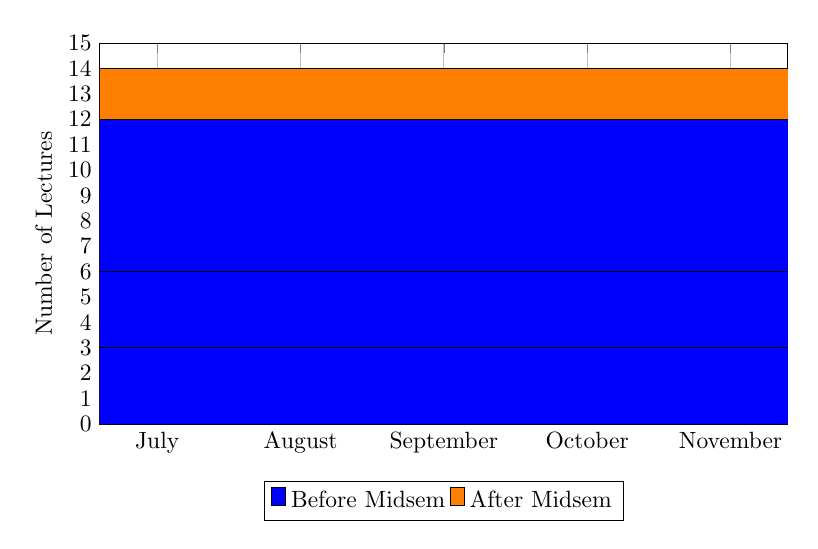
\begin{tikzpicture}[scale=0.85,transform shape]
    \begin{axis}[ybar stacked, 
                 ylabel = Number of Lectures,
                 grid = major,
                 ymin = 0,
                 ymax = 15,
                 ytick = {0,1,...,15},
                 xtick = {1,3,5,7,9},
                 xticklabels = {July,August,September,October,November},
                 %symbolic x coords={Jul,Aug,Sep,Oct,Nov},
                 legend style={at={(0.5,-0.15)}, anchor = north, legend columns=-1},
                 x post scale = 1.5
                 ]
      \addplot[fill=blue, bar width = 20] coordinates
      {(1,6) (3, 12) (5, 3) (7,0) (9,0)};
      %{(Jul,3) (Aug, 9) (Sep, 2) (Oct,0) (Nov,0)};
      \addplot[fill=orange, bar width = 20] coordinates
      {(1, 0) (3, 0) (5, 6) (7,14) (9, 4)};
      %{(Jul, 0) (Aug, 0) (Sep, 3) (Oct,8) (Nov, 5)};
    \legend{Before Midsem, After Midsem}
    \end{axis}
  \end{tikzpicture}
  \end{figure}

  \begin{description}
    \item[Before Midsem] 21 Lectures
    \item[After Midsem] 24 Lectures
    \pause
    \item[Attendance] \alert{80\% required} (Can miss at most nine lectures)
  \end{description}
\end{frame}

\begin{frame}{}
\vfill
\begin{center}
End of course outline
\end{center}
\vfill
\end{frame}
\end{document}
